\section{\LaTeX - Hilfestellung}

\begin{figure}[h]
  \centering
  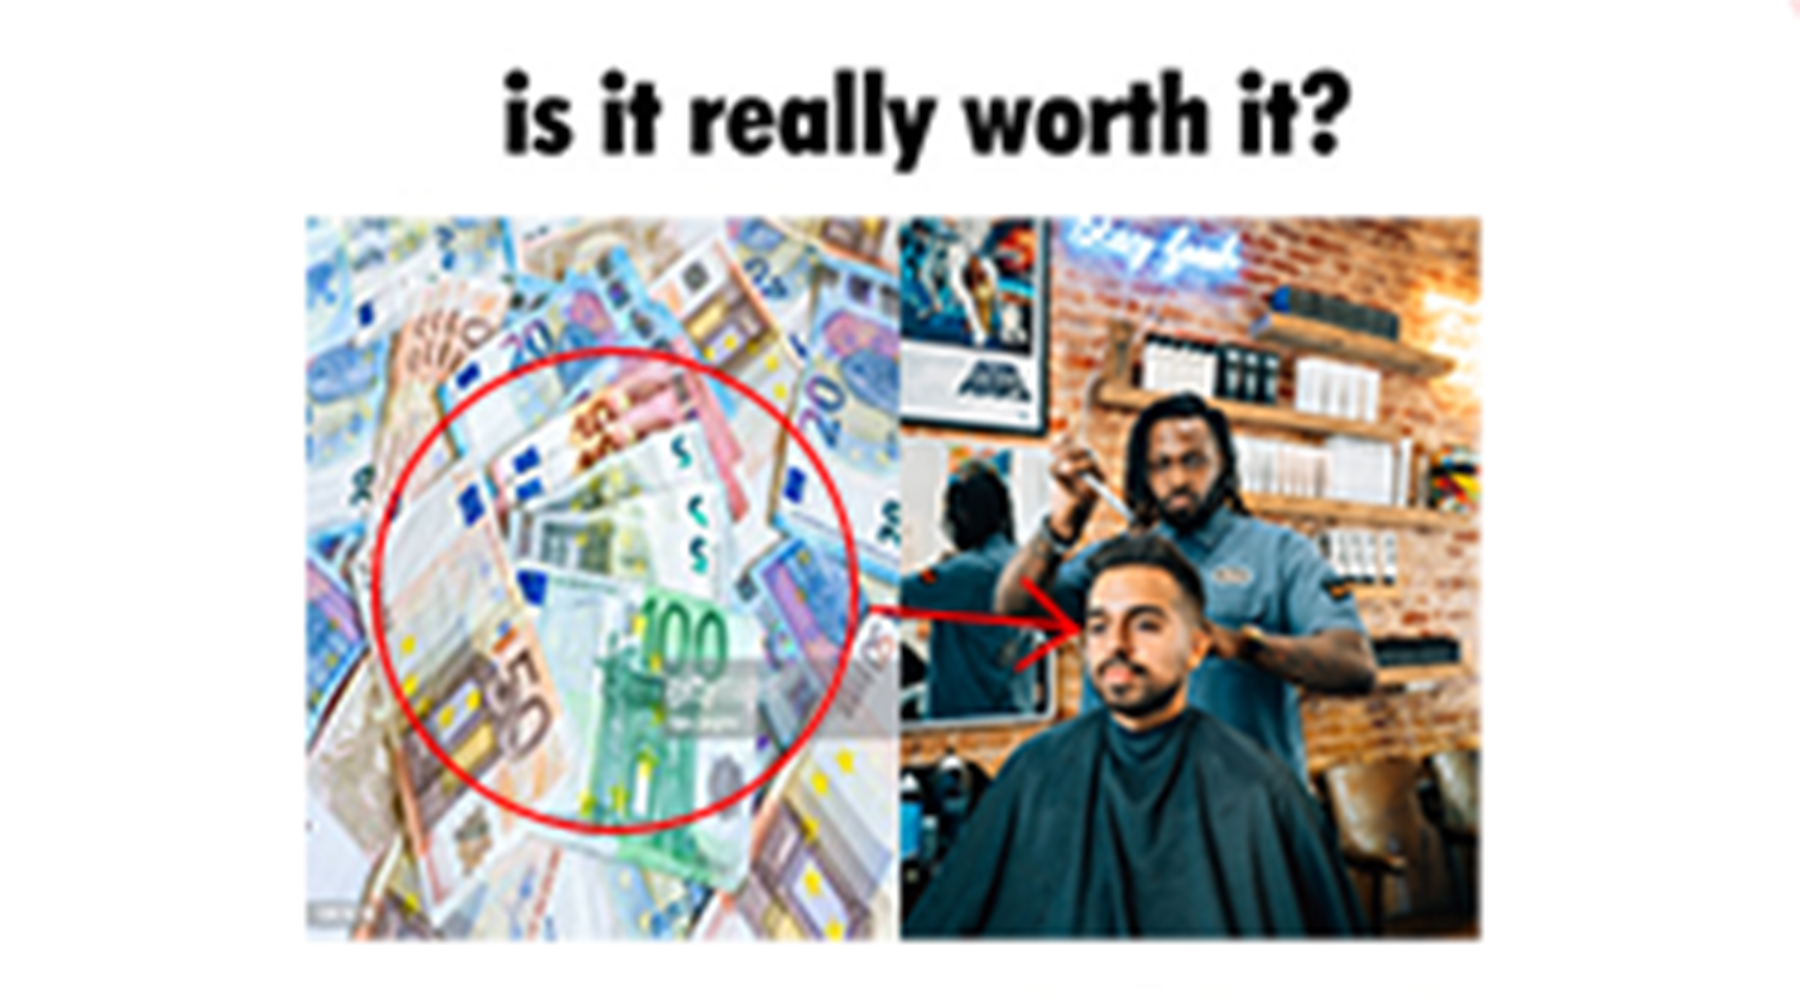
\includegraphics[width=0.75\textwidth]{images/test}
  \caption{Fahrradboxen werden von einem \ac{RBG} bedient.}
  \label{fig:fahrrad_box}
\end{figure}

\begin{table}[h]
  \begin{center}
    \begin{tabular} { |c|c|c| }
      \hline
      cell 1 & cell 2 & cell 3 \\
      \hline
      cell 4 & cell 5 & cell 6 \\
      cell 7 & cell 8 & cell 9 \\
      \hline
    \end{tabular}
    \caption{Wichtige Tabelle \cite{testbook:aaaa} und \cite{stackoverflow}}.
    \label{tab:wichtige_tabelle}
  \end{center}
\end{table}
